% !TeX spellcheck = en_US
\documentclass[a4paper]{report}
\usepackage[T1]{fontenc}
\usepackage[utf8]{inputenc}
\usepackage[english]{babel}
\usepackage{geometry}
\usepackage{graphicx}
\usepackage{subfig}
%\usepackage{lipsum}
\usepackage{verbatim}
\usepackage[table,xcdraw]{xcolor}
\geometry{a4paper,top=2.5cm,bottom=2.5cm,left=3cm,right=3cm,%
	heightrounded,bindingoffset=5mm}

\usepackage{color}
\usepackage{listings}
\usepackage{xcolor}

\usepackage{color}
\usepackage{listings}
\lstset{ %
	language=Java,                % choose the language of the code
	basicstyle=\footnotesize,       % the size of the fonts that are used for the code
	numbers=left,                   % where to put the line-numbers
	numberstyle=\footnotesize,      % the size of the fonts that are used for the line-numbers
	stepnumber=1,                   % the step between two line-numbers. If it is 1 each line will be numbered
	numbersep=5pt,                  % how far the line-numbers are from the code
	backgroundcolor=\color{white},  % choose the background color. You must add \usepackage{color}
	showspaces=false,               % show spaces adding particular underscores
	showstringspaces=false,         % underline spaces within strings
	showtabs=false,                 % show tabs within strings adding particular underscores
	frame=single,           % adds a frame around the code
	tabsize=2,          % sets default tabsize to 2 spaces
	captionpos=b,           % sets the caption-position to bottom
	breaklines=true,        % sets automatic line breaking
	breakatwhitespace=false,    % sets if automatic breaks should only happen at whitespace
	escapeinside={\%*}{*)}          % if you want to add a comment within your code
}

\newcommand{\HRule}{\rule{\linewidth}{0.5mm}}

\begin{document}
	\begin{titlepage}
		\begin{center}
			
			% Top 
			
\includegraphics[width=0.45\textwidth]{img/unipi.png}~\\[2.5cm]
			
			
			% Title
			\HRule \\[0.4cm]
			{ \LARGE 
				\textbf{Intent Based Application}\\[0.4cm]
				\emph{Group Project Report for Advanced Network Architectures And Wireless Systems}\\[0.4cm]
			}
			\HRule \\[1.5cm]
			
			
			
			% Author
			{ \large
				Francesco Iemma \\[0.1cm]
				Yuri Mazzuoli \\[0.1cm]
				Giovanni Menghini \\[0.1cm]
			}
			
			\vfill
			
			\textsc{\large M.Sc. in Computer Engineering}\\[0.4cm]
			
			
			% Bottom
			{\large Academic Year 2021/22}
			
		\end{center}
	\end{titlepage}
	
	
	\tableofcontents
	\newpage
	
	
	
	
	\chapter{Implementation}
	
	\section{Floodlight Functionalities}
	\subsection{How To Compute A Path: Routing Service}
	\subsection{How To Install A Path: Forwarding Base}
	
	
	\section{Floodlight Extended Forwarding Module}\label{forwarding}
	\noindent The main module of our package is IntentForwarding. This module is an extension of the floodlight  forwarding module\footnote{net.floodlightcontroller.forwarding.Forwarding}, in general the added functionalities are:
	
	\begin{itemize}
		\item An array list that remembers the list of active intents
		\item The extension of the method \textit{ProcessPacketInMessage} in order to check if the packet that triggered the packetIn is from two host that are allowed to communicate (an intent between the two exists) or not. 
	\end{itemize}
	

	\subsection{Intent Life Cycle}
	\noindent An intent is created, is active and then, when the time indicated in the intent establishment request finishes, expires.
	
	\noindent When an intent is created the following operations are done:
	\begin{itemize}
		\item It is checked if an intent with the same IPs already exists. If yes no other operations are performed.
		
		\item A new timeout task is created and scheduled in order to be executed in the amount of time indicated by the intent timeout
		
		\item The intent is added to the array list
	\end{itemize}
	
	\noindent Notice that the creation of the timer is needed in order to implement the intent expiration and to perform some operations when this happens.
	
	\noindent The operations that must be done when the intent expires are:
	\begin{itemize}
		\item Install rules in certain switches in order to deny the communications between the host of the expired intent
		\item Delete the intent from the intent database
	\end{itemize}

	\noindent Thus the main problem is to decide which are the switches where we have to install the rules.
	
	
	\noindent Let assume that we have two host: \textit{host1} and \textit{host2} and an intent between them exists and it is going to expire. In order to minimize the packets in the network from hosts of an expired intent it was decided to install the rules in the first switch encountered by the \textit{host1} when sends the message to \textit{host2} (we will call this switch \textit{switch1}) and in the first switch encountered when \textit{host2} sends a message to \textit{host1} (we will call this switch \textit{switch2}).
	
	
	\noindent The rules installed on each of the two switches are:
	\begin{itemize}
		\item Deny IPv4 from \textit{host1} to \textit{host2}
		\item Deny IPv4 from \textit{host2} to \textit{host1}
	\end{itemize}
	
	\noindent Both rules are valid for 5 seconds by default. See figure \ref{img:switch12_example} for a graphical representation.
	
	\begin{figure}[htp]
		\centering
		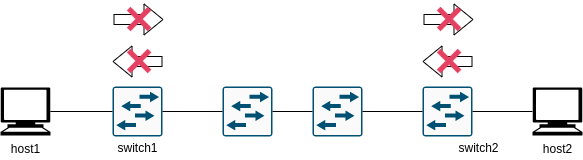
\includegraphics[width=0.7\linewidth]{img/example.png}
		\caption{Graphical representation of where the rules for denying the communications between two hosts are installed}
		\label{img:switch12_example}
	\end{figure}
	
	 \noindent Thanks to this rules no other packets are allowed to pass from \textit{switch1} and \textit{switch2} after the intent expiry. When the rules are no longer valid for each packet arriving to \textit{switch1} or \textit{switch2} a packetIn is generated and thus the \textit{ProcessPacketInMessage} method will check if that packet is allowed (an intent has been re-established) or not (the old intent has expired and no other intent have been established).
	 
	 \noindent Notice that due to the fact that the rules installed in the switches are valid for a certain time, no intent can be established until that rules are no longer valid. In the default case the rules are valid for 5 seconds and so a new intent regarding one of the two hosts can be established 5 seconds after the expiry of the old intent. That time can be changed by the network manager through REST.
	 
	 \noindent The last problems that need a solution is how we can know which is the identifier of \textit{switch1} and \textit{switch2}. When the timeout task (the task that will be performed when the intent expires) is created we pass to the constructor:
	 \begin{itemize}
	 	\item A reference to the object IntentForwarding, this is necessary in order to call the function who is in charge to install rules in the switches
	 	\item A reference to the object representing the intent associated to that timeout task. That object is \textbf{HostPair} and it is composed by:
	 	\begin{itemize}
	 		\item IPv4Address host1IP
	 		\item IOFSwitch sw1
	 		\item IPv4Address host2IP
	 		\item IOFSwitch sw2
	 		\item long timeout
	 	\end{itemize}
 		\noindent That reference is necessary in order to retrieve the identifier of \textit{switch1} and \textit{switch2}. That identifiers are set when the first packetIn coming from the first switch encountered by the packet sent by an host is handled by the extended forwarding module i.e. IntentForwarding (for more on this see \ref{sec:Ipv4}).
	 \end{itemize}
 	\noindent Here we can see the code executed when we add an intent.
 	
 	\begin{lstlisting}
 	public boolean addNewIntent(HostPair newPair) {
 		System.out.print("AddNewIntent Called\n");
 		if(intentsDB.contains(newPair)) {
 			log.info(" Intent already present in Intents List");
 			return false;
 		}
 			
 		long timeout = newPair.getTimeout();
 		Timer timer = new Timer();
 		TimerTask task = new TimeoutTask(newPair, this);
 		timer.schedule(task, timeout);
 			
 		intentsDB.add(newPair);
 		return true;
 	}
 	\end{lstlisting}
	
	\subsection{IPv4 Management}\label{sec:Ipv4}
	\noindent When a packetIn regarding an IPv4 packet arrives the operations donw are:
	\begin{itemize}
		\item The intents database is searched:
		\begin{itemize}
			\item If exists an intent between the sender and the receiver (or viceversa) then
			\begin{itemize}
				\item If the sender is \textit{host1} and \textit{switch1} in the object HostPair representing the intent, is null then \textit{switch1} is set equal to the identifier of the switch that has sent the packetIn that has triggered this execution of ProcessPacketInMessage. Same thing is done for \textit{switch2}. 
				\item Then the method of the super class (Forwarding.java) is invoked 
			\end{itemize} 
			\item Otherwise two rules are installed on the switch that sent the packetIn in order to deny the communication between the two hosts for a certain amount of time (the default timeout is 5 seconds but that value can be customized through REST API).
		\end{itemize}
	\noindent Here a section of the method \textit{processPacketInMessage}. Notice that when setting the switch id is the method \textit{setSw(IOFSwitch switch)} that checks if the switch is already set or not and set the switch only if it is not already set.
	\begin{lstlisting}
	HostPair hp = null;
	int hpIndex = intentsDB.indexOf(new HostPair(sourceIP, destinIP));
	if (hpIndex != -1)
		hp = intentsDB.get(hpIndex);
		
	if(hp != null && intentsDB.contains(hp)) {
		System.out.printf("allowing: %s - %s on switch %s \n",
			sourceIP.toString(), destinIP.toString(), sw.getId());	
		if(hp.getHost1IP().equals(sourceIP))
			hp.setSw1(sw);
		if(hp.getHost2IP().equals(sourceIP))
			hp.setSw2(sw);
		return super.processPacketInMessage(sw, pi, decision, cntx);	
	}
	denyRoute(sw, sourceIP, destinIP);
	denyRoute(sw, destinIP,sourceIP);
	return Command.CONTINUE;
	\end{lstlisting}
	\end{itemize}


	\subsection{ARP Management}
	\noindent The ARP protocol is used to retrieve the layer 2 address of an host given its IP address. When an ARP packet arrives to a switch a packetIn is sent to the controller and so the processPacketInMessagge is invoked, the method understands that the packet that has triggered the packetIn is an ARP packet and so it must be handled differently.
	\noindent The first operation done is checking if an intent between the sender and the receiver exists using their IPs. If an intent exists then the method of the super class is invoked otherwise the ARP packet is blocked. The rules to avoid communication between the MACs address carried inside the ARP packet are installed only if that packet is an ARP response, in that case the target MAC address is not 00:00:00:00:00:00. In fact installing a rule that deny to send an ARP messagge from a certain mac X to 00:00:00:00:00:00 means deny X to runs the ARP protocol because for each ARP request the target mac is 00:00:00:00:00:00 i.e. unspecified mac.
	
	
	\section{REST API For Establishing An Intent}
	\section{Responsiveness To Link Failures \& Topology Changes}
	\chapter{Testing}
	
\end{document}
